\documentclass[UTF8,a4paper,11pt]{ctexart}

% ── Page geometry ──
\usepackage[margin=2.2cm,top=2.5cm,bottom=2.5cm]{geometry}

% ── Typography & math ──
\usepackage{fontspec}
\usepackage{amsmath,amssymb}
\usepackage{setspace}
\setstretch{1.25}

% ── Graphics ──
\usepackage{tikz}
\usetikzlibrary{arrows.meta,calc,positioning}

% ── Colors ──
\usepackage{xcolor}
\definecolor{accent}{HTML}{1a73e8}
\definecolor{darkgray}{HTML}{333333}
\definecolor{lightgray}{HTML}{f5f5f5}
\definecolor{notebg}{HTML}{e8f0fe}
\definecolor{warnbg}{HTML}{fef7e0}
\definecolor{calcbg}{HTML}{e6f4ea}
\definecolor{calcframe}{HTML}{188038}

% ── Links ──
\usepackage{hyperref}
\hypersetup{colorlinks=true,linkcolor=accent,urlcolor=accent}

% ── Layout ──
\usepackage{enumitem}
\setlist[itemize]{leftmargin=1.8em,itemsep=2pt}
\setlist[enumerate]{leftmargin=1.8em,itemsep=2pt}
\usepackage{booktabs}
\usepackage{tcolorbox}
\usepackage{titlesec}
\usepackage{fancyhdr}
\usepackage{lastpage}

% ── Header/Footer ──
\pagestyle{fancy}
\fancyhf{}
\fancyhead[L]{\small\textcolor{darkgray}{高中数学必修一 · 九天核心概念讲义}}
\fancyhead[R]{\small\textcolor{darkgray}{从第一性原理理解集合、函数与三角}}
\fancyfoot[C]{\small\textcolor{darkgray}{\thepage\ / \pageref{LastPage}}}
\renewcommand{\headrulewidth}{0.4pt}

% ── Section styling ──
\titleformat{\section}
  {\Large\bfseries\color{accent}}
  {\thesection}{1em}{}
\titleformat{\subsection}
  {\large\bfseries\color{darkgray}}
  {\thesubsection}{1em}{}

% ── Custom boxes ──
\newtcolorbox{keyconcept}[1][]{
  colback=notebg, colframe=accent,
  fonttitle=\bfseries, boxrule=0.5pt,
  left=8pt, right=8pt, top=6pt, bottom=6pt, title={#1}}
\newtcolorbox{exercise}[1][]{
  colback=warnbg, colframe=orange,
  fonttitle=\bfseries, boxrule=0.5pt,
  left=8pt, right=8pt, top=6pt, bottom=6pt, title={#1}}
\newtcolorbox{calcbox}[1][]{
  colback=calcbg, colframe=calcframe,
  fonttitle=\bfseries, boxrule=0.5pt,
  left=8pt, right=8pt, top=6pt, bottom=6pt, title={#1}}

\newcommand{\daytitle}[2]{%
  \section*{#1\quad #2}%
  \addcontentsline{toc}{section}{#1\quad #2}}

\begin{document}

% ═══ 封面 ═══
\begin{center}
  \vspace*{2cm}
  {\Huge\bfseries\color{accent} 高中数学必修一}\\[0.4cm]
  {\LARGE 九天核心概念讲义}\\[1.2cm]
  {\large 写给准高中生：从第一性原理理解集合、函数与三角}\\[0.5cm]
  {\small\textcolor{darkgray}{依据：普通高中教科书《数学》必修第一册（人教 A 版，2017 课标）}}\\[0.3cm]
  {\small\textcolor{darkgray}{\today}}
  \vfill
  {\small 每天 60–90 分钟：先读讲解，再合上讲义把概念讲出来，最后做自测。}
\end{center}
\newpage

\tableofcontents
\newpage

% ═══ 使用说明 ═══
\section*{开始前：这本讲义在做什么}
\addcontentsline{toc}{section}{开始前：这本讲义在做什么}

必修一共五章，是一条不断升级的线：

\begin{enumerate}
  \item \textbf{语言}（第一章）：集合与常用逻辑用语——把数学陈述写得没有歧义；
  \item \textbf{工具}（第二章）：不等式——特别是基本不等式和二次不等式，是高中解题的硬通货；
  \item \textbf{主角}（第三、四章）：函数——用集合语言重新定义，再研究性质（单调、奇偶），最后落进三个具体家族（幂、指数、对数）；
  \item \textbf{新朋友}（第五章）：三角函数——第一支描写"周而复始"的函数，从单位圆里长出来。
\end{enumerate}

它在初中数学之上，真正新增的是三样东西：

\begin{keyconcept}[九天要带走的三样工具]
\begin{itemize}
  \item \textbf{精确语言}：集合符号（$\in$、$\subseteq$、$\cap$、$\cup$、区间）+ 逻辑用语（充分必要、$\forall$、$\exists$）。高中数学的每个定义都用它书写。
  \item \textbf{函数的对应观}：函数是"每个输入对应唯一输出"的规则。定义域、对应法则、值域三要素，以及用"任意"写出的严格定义（单调性、奇偶性）。
  \item \textbf{三大家族 + 一支周期函数}：指数、对数、幂函数描写增长；三角函数描写周期。对数是指数的反解，三角是单位圆上点的坐标——理解这两条，公式基本不用背。
\end{itemize}
\end{keyconcept}

\textbf{每天的学习流程}（60–90 分钟）：
\begin{enumerate}
  \item 读当天的讲解，重点看"为什么这样定义"，不要背结论；
  \item 合上讲义，把当天的核心概念\textbf{讲给别人听}（或讲给自己听），卡壳的地方就是没懂的地方；
  \item 做"今日自测"，对照书末的答案。
\end{enumerate}

\newpage

% ═══ 第 1 天 ═══
\daytitle{第 1 天}{集合与逻辑：数学的精确语言}

\textbf{核心问题}：怎样毫无歧义地谈论"一群对象"，以及"谁推出谁"？

\subsection*{1.1 为什么发明集合}

看两句话："本班身高较高的同学""本班身高超过 175 cm 的同学"。第一句话没法执行——什么叫"较高"？第二句话人人能执行，因为成员资格有明确标准。\textbf{集合就是把"一群对象"说清楚的方式}：把一些确定的、不同的对象组成的总体叫做集合，对象叫元素。

\begin{keyconcept}[集合中元素的三个特性]
\begin{itemize}
  \item \textbf{确定性}：每个对象"在不在里面"必须有明确答案。"身材较高的人"不能构成集合。
  \item \textbf{互异性}：同一个元素只算一次，$\{1,1,2\}$ 就是 $\{1,2\}$。
  \item \textbf{无序性}：$\{1,2,3\}$ 与 $\{3,2,1\}$ 是同一个集合。
\end{itemize}
\end{keyconcept}

两种写法：\textbf{列举法} $\{1,2,3\}$（适合有限、少的）；\textbf{描述法} $\{x \in \mathbb{R} \mid x > 3\}$（竖线右边是"入场条件"）。常用数集有专用字母：$\mathbb{N}$（自然数）、$\mathbb{Z}$（整数）、$\mathbb{Q}$（有理数）、$\mathbb{R}$（实数）。元素与集合的关系用 $\in$ / $\notin$。

如果集合 $A$ 的元素都在 $B$ 里，就说 $A$ 是 $B$ 的\textbf{子集}，记 $A \subseteq B$。注意：任何集合都是自己的子集；\textbf{空集 $\varnothing$ 是任何集合的子集}。

三种基本运算，对应三个日常逻辑词：

\begin{keyconcept}[交、并、补 = 且、或、不]
\begin{itemize}
  \item \textbf{交集} $A \cap B$：既在 $A$ \textbf{且}在 $B$ 中的元素；
  \item \textbf{并集} $A \cup B$：在 $A$ \textbf{或}在 $B$ 中的元素（合起来，重复只算一次）；
  \item \textbf{补集} $\complement_U A$：在全集 $U$ 中\textbf{不}在 $A$ 中的元素。
\end{itemize}
\end{keyconcept}

\begin{center}
\begin{tikzpicture}[scale=1.0]
  % A∩B
  \begin{scope}[xshift=0cm]
    \clip (0,0) circle (1.1);
    \fill[accent!25] (1.3,0) circle (1.1);
  \end{scope}
  \draw[thick] (0,0) circle (1.1) node at (-0.65,0.85) {$A$};
  \draw[thick] (1.3,0) circle (1.1) node at (1.95,0.85) {$B$};
  \node at (0.65,-1.55) {$A \cap B$（阴影）};
  % A∪B
  \begin{scope}[xshift=4.6cm]
    \fill[accent!25] (0,0) circle (1.1);
    \fill[accent!25] (1.3,0) circle (1.1);
  \end{scope}
  \draw[thick] (4.6,0) circle (1.1) node at (3.95,0.85) {$A$};
  \draw[thick] (5.9,0) circle (1.1) node at (6.55,0.85) {$B$};
  \node at (5.25,-1.55) {$A \cup B$（阴影）};
  % 补集
  \fill[accent!25] (8.3,-1.4) rectangle (11.5,1.4);
  \fill[white] (9.6,0) circle (0.95);
  \draw[thick,darkgray] (8.3,-1.4) rectangle (11.5,1.4);
  \draw[thick] (9.6,0) circle (0.95) node {$A$};
  \node at (11.1,1.05) {$U$};
  \node at (9.9,-1.8) {$\complement_U A$（阴影）};
\end{tikzpicture}
\end{center}

\begin{keyconcept}[最容易踩的两个坑]
\begin{itemize}
  \item $\in$ 与 $\subseteq$ 不能混用：$\in$ 连接\textbf{元素与集合}（$1 \in \{1,2\}$），$\subseteq$ 连接\textbf{集合与集合}（$\{1\} \subseteq \{1,2\}$）。
  \item $\varnothing$、$\{0\}$、$\{\varnothing\}$ 是三个不同的东西：空集、装了一个 0 的集合、装了一个空集的集合。
\end{itemize}
\end{keyconcept}

\subsection*{1.2 充分条件与必要条件：谁推出谁}

数学命题大多是"若 $p$，则 $q$"。如果 $p$ 成立能\textbf{推出} $q$ 成立（记 $p \Rightarrow q$），就说 $p$ 是 $q$ 的\textbf{充分条件}，$q$ 是 $p$ 的\textbf{必要条件}。两个方向都成立（$p \Leftrightarrow q$），就是\textbf{充要条件}。

记法总是绕，用集合观点一眼看穿：把条件看成集合，

\[
p \Rightarrow q \quad\Longleftrightarrow\quad P \subseteq Q
\]

\textbf{小范围推大范围}：$x > 3$ 的集合是 $x > 1$ 的子集，所以 $x > 3 \Rightarrow x > 1$（$x>3$ 是 $x>1$ 的充分条件），但反过来推不出。范围越小条件越"充分"，范围越大条件越"必要"。

\subsection*{1.3 全称量词与存在量词}

数学要说"所有"和"存在"，各有一个符号：$\forall$（任意，All 倒写）、$\exists$（存在，Exist 反写）。

最重要的是\textbf{怎么否定}它们——考试和证明里天天用：

\begin{keyconcept}[含量词命题的否定：改量词，否结论]
\begin{itemize}
  \item "所有奇数都是素数"（$\forall$）的否定是"\textbf{存在一个}奇数不是素数"（$\exists$）——原命题假，否定真（9 就是反例）。
  \item "存在一个实数 $x$ 使 $x^2 < 0$"（$\exists$）的否定是"\textbf{所有}实数都满足 $x^2 \geq 0$"（$\forall$）。
\end{itemize}
规则只有一条：否定把 $\forall$ 换成 $\exists$、$\exists$ 换成 $\forall$，再否定结论。这正是第 3 天要讲的"任意 vs 反例"：证明全称命题需要对所有 $x$ 成立，推翻它只要一个反例。
\end{keyconcept}

\begin{exercise}[今日自测]
\begin{enumerate}
  \item 设 $A = \{1,2,3\}$，$B = \{2,3,4\}$，全集 $U = \{1,2,3,4,5\}$。求 $A \cap B$、$A \cup B$、$\complement_U A$。
  \item "$x$ 是 6 的倍数"是"$x$ 是 3 的倍数"的什么条件？（充分/必要/充要/都不是）
  \item 写出命题"所有正方形都是矩形"的否定，并判断真假。
\end{enumerate}
\end{exercise}

\newpage

% ═══ 第 2 天 ═══
\daytitle{第 2 天}{不等式：作差法、基本不等式与二次不等式}

\textbf{核心问题}：怎样比较两个量的大小，怎样求"最省""最大"？

\subsection*{2.1 比较大小只有一个办法：作差}

等式的性质初中就熟（两边同加同乘仍相等）。不等式多一条"脾气"：\textbf{两边同乘负数，不等号要转向}。其余都类似：同加不变向，同乘正数不变向。

比较两个式子谁大，高中只用一个原理：
\[
a > b \iff a - b > 0
\]
把"比大小"转化成"作差后判断正负"——这就是\textbf{作差比较法}，第 3 章证明单调性用的还是它。

\subsection*{2.2 基本不等式：从 $(a-b)^2 \geq 0$ 长出来}

任何实数的平方非负：$(a-b)^2 \geq 0$，展开得 $a^2 + b^2 \geq 2ab$。把 $a$、$b$ 换成 $\sqrt{a}$、$\sqrt{b}$（要求 $a, b > 0$），立刻得到：

\begin{keyconcept}[基本不等式]
\[
\frac{a+b}{2} \geq \sqrt{ab} \qquad (a > 0,\ b > 0)
\]
当且仅当 $a = b$ 时取等号。左边是\textbf{算术平均}，右边是\textbf{几何平均}。
\end{keyconcept}

它不是孤立的公式，是"平方非负"这条第一性原理的直接推论——自己推一遍，就不用背。几何上它同样显然：

\begin{center}
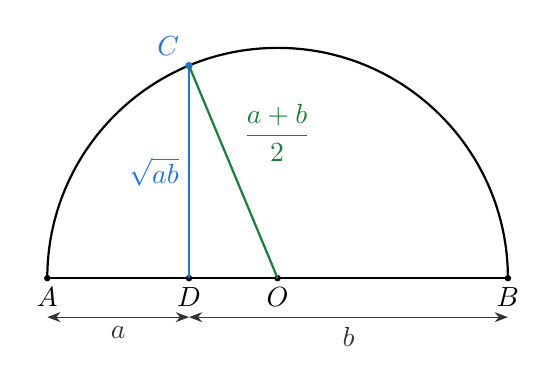
\begin{tikzpicture}[>=Stealth,scale=0.9]
  % 半圆：直径 a+b = 2+4.5 = 6.5，圆心 (3.25,0)，半径 3.25
  \draw[thick] (0,0) arc (180:0:3.25);
  \draw[thick] (0,0) -- (6.5,0);
  \fill (0,0) circle (1.3pt) node[below] {$A$};
  \fill (6.5,0) circle (1.3pt) node[below] {$B$};
  \fill (3.25,0) circle (1.3pt) node[below] {$O$};
  \fill (2,0) circle (1.3pt) node[below] {$D$};
  % C 在半圆上，x=2：y = sqrt(3.25^2 - 1.25^2) = 3
  \fill[accent] (2,3) circle (1.5pt) node[above left] {$C$};
  \draw[thick,accent] (2,0) -- (2,3) node[midway,left] {$\sqrt{ab}$};
  \draw[thick,calcframe] (3.25,0) -- (2,3) node[midway,above right] {$\dfrac{a+b}{2}$};
  \draw[<->,darkgray] (0,-0.55) -- (2,-0.55) node[midway,below] {$a$};
  \draw[<->,darkgray] (2,-0.55) -- (6.5,-0.55) node[midway,below] {$b$};
\end{tikzpicture}
\end{center}

直径上 $AD = a$、$DB = b$，竖起的半弦 $CD = \sqrt{ab}$，半径 $OC = \dfrac{a+b}{2}$。半径是圆里最长的"半弦方向"，所以 $\dfrac{a+b}{2} \geq \sqrt{ab}$；只有当 $D$ 与 $O$ 重合（$a = b$）时两者相等。

\begin{keyconcept}[用它来求最值：两个口诀]
\begin{itemize}
  \item \textbf{积定和最小}：$ab$ 固定时，$a+b \geq 2\sqrt{ab}$，$a = b$ 时和最小；
  \item \textbf{和定积最大}：$a+b$ 固定时，$\sqrt{ab} \leq \dfrac{a+b}{2}$，$a = b$ 时积最大。
\end{itemize}
例：用 20 m 篱笆围矩形菜地，什么时候面积最大？$2(a+b)=20$，和定，$a=b=5$（正方形）时面积最大 25 m$^2$。
\end{keyconcept}

\subsection*{2.3 二次不等式：看图，不背表}

解 $x^2 - 4x + 3 < 0$。别背口诀，画抛物线 $y = x^2 - 4x + 3 = (x-1)(x-3)$：开口向上，与 $x$ 轴交于 $x=1$、$x=3$。不等式问的是"\textbf{$y$ 什么时候为负}"——看图：两根之间。

\begin{center}
\begin{tikzpicture}[>=Stealth,scale=0.95]
  \draw[->] (-0.8,0) -- (5.0,0) node[right] {$x$};
  \draw[->] (0,-1.6) -- (0,2.6) node[above] {$y$};
  \fill[accent!15] plot[domain=1:3,samples=30] (\x,{\x*\x-4*\x+3}) -- (3,0) -- (1,0) -- cycle;
  \draw[very thick,accent] plot[domain=0.1:3.9,samples=50] (\x,{\x*\x-4*\x+3});
  \fill (1,0) circle (1.5pt) node[above left] {$1$};
  \fill (3,0) circle (1.5pt) node[above right] {$3$};
  \node[darkgray] at (2,-0.55) {$y<0$：$1<x<3$};
  \node[accent] at (4.35,1.6) {$y=(x-1)(x-3)$};
\end{tikzpicture}
\end{center}

判别式 $\Delta$ 决定抛物线与 $x$ 轴的关系：$\Delta > 0$ 两个交点，$\Delta = 0$ 相切，$\Delta < 0$ 不相交（开口向上时恒在上方，$y < 0$ 无解）。\textbf{二次函数、二次方程、二次不等式是同一个对象的三张面孔}：方程找的是交点，不等式问的是图象在轴上方还是下方。

\begin{exercise}[今日自测]
\begin{enumerate}
  \item 已知 $a > b$，比较 $-2a + 1$ 与 $-2b + 1$ 的大小，并说明理由。
  \item 求 $x + \dfrac{1}{x}$（$x > 0$）的最小值，以及取到最小值时的 $x$。
  \item 解不等式 $x^2 - 4x + 3 > 0$ 和 $x^2 + x + 1 < 0$。
\end{enumerate}
\end{exercise}

\newpage
% ═══ 第 3 天 ═══
\daytitle{第 3 天}{函数：从"变量"到"对应"}

\textbf{核心问题}：$y = x^2$ 和"每个输入对应它的平方"，为什么是两种层次的理解？

\subsection*{3.1 函数的新定义}

初中说："$y$ 随 $x$ 的变化而变化，$y$ 是 $x$ 的函数。"这话没错，但没法回答这些问题：$y = 1$（常数）是函数吗？圆周率 $\pi$ 能是某个函数的输出吗？高中用集合语言给了一个更硬朗的定义：

\begin{keyconcept}[函数（对应说）]
设 $A$、$B$ 是两个\textbf{非空数集}。如果按照某种对应法则 $f$，$A$ 中的\textbf{每一个}元素 $x$，在 $B$ 中都有\textbf{唯一}的元素 $y$ 与它对应，就称 $f: A \to B$ 为从 $A$ 到 $B$ 的函数，记 $y = f(x)$。

三个关键词：\textbf{每一个}（$A$ 中不许有漏网的）、\textbf{唯一}（一个输入只许一个输出）、\textbf{数集}（本册只研究数到数的对应）。
\end{keyconcept}

\begin{center}
\begin{tikzpicture}[>=Stealth,scale=1.0]
  \draw[thick] (0,0) ellipse (1.0 and 1.7);
  \node at (0,2.1) {$A$（定义域）};
  \draw[thick] (4.5,0) ellipse (1.0 and 1.7);
  \node at (4.5,2.1) {$B$};
  \fill (0,0.9) circle (1.5pt) node[left] {$x_1$};
  \fill (0,0) circle (1.5pt) node[left] {$x_2$};
  \fill (0,-0.9) circle (1.5pt) node[left] {$x_3$};
  \fill (4.5,0.9) circle (1.5pt) node[right] {$y_1$};
  \fill (4.5,-0.2) circle (1.5pt) node[right] {$y_2$};
  \draw[->,thick,accent] (0.25,0.9) -- (4.2,0.9);
  \draw[->,thick,accent] (0.25,0) -- (4.2,-0.2);
  \draw[->,thick,accent] (0.25,-0.9) -- (4.2,-0.25);
  \node[accent] at (2.25,1.3) {$f$（对应法则）};
  \node[darkgray] at (4.5,-2.2) {$f$ 的值域 $\subseteq B$（允许多个 $x$ 指向同一个 $y$）};
\end{tikzpicture}
\end{center}

函数的\textbf{三要素}：定义域、对应法则、值域。两个函数"相同"，当且仅当定义域和对应法则都相同——所以 $f(x) = x$（$x \in \mathbb{R}$）与 $g(x) = \dfrac{x^2}{x}$ \textbf{不是}同一个函数：后者 $x$ 不能取 0。

\subsection*{3.2 f(x) 记号与区间}

$f(x)$ 读作"$f$ 在 $x$ 处的值"：$f$ 是规则本身，$x$ 是输入，$f(x)$ 是输出。$f(2)$ 不是乘法，是"把 2 送进规则 $f$"。

定义域常用\textbf{区间}书写：$[a,b]$ 含端点（闭），$(a,b)$ 不含（开），$[a,+\infty)$ 表示 $x \geq a$。比如 $f(x) = \sqrt{x-1}$ 的定义域是 $[1,+\infty)$，因为根号里的量必须非负——\textbf{求定义域就是排查"哪些输入会让规则死机"}：分母为 0、负数开偶次方。

\begin{exercise}[今日自测]
\begin{enumerate}
  \item $y = 1$（常数函数）符合函数定义吗？用"每一个、唯一"检验。
  \item 求 $f(x) = \dfrac{1}{x-2} + \sqrt{x}$ 的定义域（用区间表示）。
  \item $f(x) = x^2$ 与 $g(t) = t^2$ 是同一个函数吗？$h(x) = |x|$ 与 $p(x) = \sqrt{x^2}$ 呢？
\end{enumerate}
\end{exercise}

\newpage

% ═══ 第 4 天 ═══
\daytitle{第 4 天}{函数的性质：单调性、奇偶性与幂函数}

\textbf{核心问题}："图象在上升"人人会看——但怎样\textbf{证明}？对称又怎样精确刻画？

\subsection*{4.1 单调性：第一个严格定义}

初中描述"$y$ 随 $x$ 增大而增大"靠的是看图。看图有用，但图只能画出函数的一小段、有限个点。高中的做法是把直观翻译成一条可检验的严格定义：

\begin{keyconcept}[单调性的定义]
设函数 $f(x)$ 的定义域为 $D$，区间 $I \subseteq D$。如果对于 $I$ 内\textbf{任意}两个自变量的值 $x_1, x_2$，当 $x_1 < x_2$ 时，都有
\[
f(x_1) < f(x_2)
\]
就说 $f(x)$ 在区间 $I$ 上是\textbf{增函数}（若都有 $f(x_1) > f(x_2)$，则是\textbf{减函数}）。

灵魂在\textbf{任意}两个字：不是挑两个点看看，而是无论取哪两个点都成立。举一万个例子也不能证明，找到一个反例就足以推翻——这正是第 1 天全称量词的逻辑。
\end{keyconcept}

\begin{center}
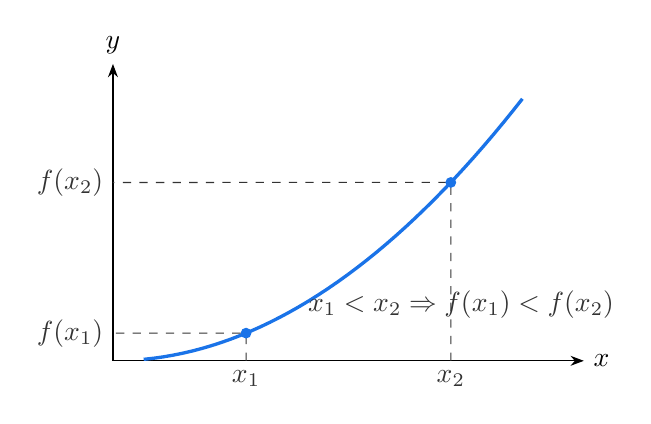
\begin{tikzpicture}[>=Stealth,scale=1.3]
  \draw[->] (0,0) -- (4.6,0) node[right] {$x$};
  \draw[->] (0,0) -- (0,2.9) node[above] {$y$};
  \draw[very thick,accent] plot[domain=0.3:4.0,samples=40] (\x,{0.16*\x*\x});
  \coordinate (X1) at (1.3,0); \coordinate (X2) at (3.3,0);
  \coordinate (P1) at (1.3,{0.16*1.69});
  \coordinate (P2) at (3.3,{0.16*10.89});
  \draw[dashed,darkgray] (X1) node[below] {$x_1$} -- (P1) -- (0,{0.16*1.69}) node[left] {$f(x_1)$};
  \draw[dashed,darkgray] (X2) node[below] {$x_2$} -- (P2) -- (0,{0.16*10.89}) node[left] {$f(x_2)$};
  \fill[accent] (P1) circle (1.5pt); \fill[accent] (P2) circle (1.5pt);
  \node[darkgray] at (3.4,0.55) {$x_1<x_2 \Rightarrow f(x_1)<f(x_2)$};
\end{tikzpicture}
\end{center}

\textbf{证明单调性的标准动作}（例：证明 $f(x) = x^2$ 在 $[0,+\infty)$ 上是增函数）：
\begin{enumerate}
  \item \textbf{取值}：任取 $x_1, x_2 \in [0,+\infty)$，且 $x_1 < x_2$；
  \item \textbf{作差}：$f(x_1) - f(x_2) = x_1^2 - x_2^2 = (x_1+x_2)(x_1-x_2)$；
  \item \textbf{定号}：$x_1+x_2 > 0$，$x_1 - x_2 < 0$，乘积 $< 0$；
  \item \textbf{结论}：$f(x_1) < f(x_2)$，所以是增函数。
\end{enumerate}
取值 $\rightarrow$ 作差 $\rightarrow$ 变形 $\rightarrow$ 定号 $\rightarrow$ 结论——注意"作差定号"就是第 2 天的作差比较法。

如果存在 $x_0 \in D$，使对任意 $x \in D$ 都有 $f(x) \leq f(x_0)$（或 $\geq$），$f(x_0)$ 就是\textbf{最大（小）值}。单调函数在闭区间上的最值一定在端点处取得。

\subsection*{4.2 奇偶性：用等式刻画对称}

有些函数的图象天生对称。对称不是"看起来美"，而是可以用等式精确刻画的性质——前提是定义域先关于原点对称（$x$ 能取，$-x$ 也必须能取）：

\begin{keyconcept}[奇偶性的定义]
\begin{itemize}
  \item \textbf{偶函数}：对定义域内任意 $x$，$f(-x) = f(x)$。图象关于 \textbf{$y$ 轴}对称（如 $f(x)=x^2$）。
  \item \textbf{奇函数}：对定义域内任意 $x$，$f(-x) = -f(x)$。图象关于\textbf{原点}对称（如 $f(x)=x^3$）。
\end{itemize}
判断三步走：\textbf{先看定义域}是否关于原点对称（不对称直接"非奇非偶"）$\rightarrow$ 求 $f(-x)$ $\rightarrow$ 与 $f(x)$、$-f(x)$ 比较。
\end{keyconcept}

\begin{center}
\begin{tikzpicture}[>=Stealth,scale=0.85]
  % 偶函数 y = x^2
  \begin{scope}[xshift=0cm]
    \draw[->] (-2.6,0) -- (2.6,0) node[right] {$x$};
    \draw[->] (0,-0.4) -- (0,3.1) node[above] {$y$};
    \draw[very thick,accent] plot[domain=-2.2:2.2,samples=40] (\x,{0.55*\x*\x});
    \node at (0,-0.9) {$f(x)=x^2$（偶：关于 $y$ 轴）};
  \end{scope}
  % 奇函数 y = x^3
  \begin{scope}[xshift=7.2cm]
    \draw[->] (-2.6,0) -- (2.6,0) node[right] {$x$};
    \draw[->] (0,-2.4) -- (0,2.6) node[above] {$y$};
    \draw[very thick,accent] plot[domain=-1.65:1.65,samples=40] (\x,{0.45*\x*\x*\x});
    \node at (0,-2.9) {$f(x)=x^3$（奇：关于原点）};
  \end{scope}
\end{tikzpicture}
\end{center}

实用价值：\textbf{对称性让工作量减半}——知道偶函数在 $x \geq 0$ 时的图象与性质，$x<0$ 的一半直接镜像出来。

\subsection*{4.3 幂函数：一个家族的第一张合影}

形如 $y = x^{\alpha}$（$\alpha$ 为常数）的函数叫\textbf{幂函数}。你已经认识它的一半家族：$y = x$（$\alpha=1$）、$y = x^2$、$y = x^{-1}$（反比例）、$y = x^3$、$y = x^{1/2}=\sqrt{x}$。

把它们的第一象限图象画在一起，规律立刻浮现：
\begin{itemize}
  \item 都过点 $(1,1)$（$1$ 的任何次幂都是 $1$）；
  \item $\alpha > 0$ 时过原点、第一象限内递增；$\alpha < 0$ 时不过原点、第一象限内递减；
  \item 奇偶性各不相同：$x^2$ 偶、$x^3$ 奇、$\sqrt{x}$ 非奇非偶（定义域 $[0,+\infty)$ 不对称）。
\end{itemize}

幂函数是后两天主角的"对照组"：\textbf{幂函数是自变量在底数上，指数函数是自变量在指数上}——位置一换，性格全变。

\begin{exercise}[今日自测]
\begin{enumerate}
  \item 用定义证明 $f(x) = -2x + 1$ 在 $\mathbb{R}$ 上是减函数。
  \item 判断 $f(x) = x^4 + x^2$、$g(x) = x^3 + x$、$h(x) = x^2 + x$ 的奇偶性。
  \item 幂函数 $y = x^{\alpha}$ 的图象都过哪个定点？为什么？
\end{enumerate}
\end{exercise}

\newpage
% ═══ 第 5 天 ═══
\daytitle{第 5 天}{指数函数：把指数从整数推向全体实数}

\textbf{核心问题}：$2^3$ 好懂，$2^{\sqrt{2}}$ 是什么意思？

\subsection*{5.1 指数幂的扩张史}

初中学过正整数指数幂：$2^3 = 2\times2\times2$。但"连乘 $\sqrt{2}$ 次"毫无意义，所以数学家换了一种定义方式——\textbf{不按"连乘"定义，而按"运算规则不变"定义}：无论指数取什么值，都要保住
\[
a^m \cdot a^n = a^{m+n}, \qquad (a^m)^n = a^{mn}, \qquad a>0
\]
用规则反推含义：
\begin{itemize}
  \item $a^0$：由 $a^0 \cdot a^n = a^n$ 得 $a^0 = 1$；
  \item $a^{-n}$：由 $a^{-n} \cdot a^n = a^0 = 1$ 得 $a^{-n} = \dfrac{1}{a^n}$；
  \item $a^{1/n}$：由 $(a^{1/n})^n = a$ 得 $a^{1/n} = \sqrt[n]{a}$（$n$ 次方根）；于是 $a^{m/n} = \sqrt[n]{a^m}$；
  \item $a^{\sqrt{2}}$：用有理数序列 $1.4, 1.41, 1.414, \dots$ 的幂无限逼近——又是一个"极限逼近"的思想（和物理讲义里瞬时速度的构造同款）。
\end{itemize}

\begin{calcbox}[数学推广的第一性原理]
数学对象的"扩军"——数从自然数到实数、指数从整数到实数——靠的都是同一条原则：\textbf{保住旧规则，扩展新领地}。定义不是被"发现"的，是被"设计"的；评价一个定义好坏的标准，是它能否让旧定理在新世界继续成立。
\end{calcbox}

\subsection*{5.2 指数函数 $y = a^x$}

\begin{keyconcept}[指数函数及其性质]
$y = a^x$（$a > 0$ 且 $a \neq 1$）：
\begin{itemize}
  \item 定义域 $\mathbb{R}$，值域 $(0, +\infty)$（正数的任何实数次幂都是正的）；
  \item 图象恒过点 $(0, 1)$（$a^0 = 1$）；
  \item $a > 1$：在 $\mathbb{R}$ 上递增（越涨越猛）；$0 < a < 1$：递减（越衰减越平缓）。
\end{itemize}
\end{keyconcept}

\begin{center}
\begin{tikzpicture}[>=Stealth,scale=0.95]
  \draw[->] (-3.4,0) -- (3.4,0) node[right] {$x$};
  \draw[->] (0,-0.4) -- (0,4.4) node[above] {$y$};
  \draw[very thick,accent] plot[domain=-3:2,samples=50] (\x,{exp(0.6931*\x)});
  \node[accent] at (2.35,3.4) {$y=2^x$};
  \draw[very thick,calcframe] plot[domain=-2:3,samples=50] (\x,{exp(-0.6931*\x)});
  \node[calcframe] at (-2.4,3.4) {$y=\left(\frac12\right)^x$};
  \fill (0,1) circle (1.5pt) node[below right=0pt and -2pt] {$(0,1)$};
  \node[darkgray] at (0,-1.0) {两图象关于 $y$ 轴对称：$\left(\frac12\right)^x = 2^{-x}$};
\end{tikzpicture}
\end{center}

指数增长的直觉：一张 0.1 mm 的纸对折 27 次，厚度约 $0.1 \times 2^{27}$ mm $\approx 13$ 公里——超过珠穆朗玛峰。线性增长是"每次加一个固定量"，指数增长是"每次乘一个固定比"，时间一长，乘法必胜。

\begin{exercise}[今日自测]
\begin{enumerate}
  \item 计算：$8^{2/3}$；$16^{-1/2}$；$\left(\dfrac{1}{2}\right)^{-3}$。
  \item 比较大小：$1.7^{0.3}$ 与 $1.7^{0.5}$；$0.8^{0.3}$ 与 $0.8^{0.5}$。（用单调性，不用计算器）
  \item 指数函数 $y = a^x$ 的值域为什么不含 0 和负数？
\end{enumerate}
\end{exercise}

\newpage

% ═══ 第 6 天 ═══
\daytitle{第 6 天}{对数函数：指数方程的反解}

\textbf{核心问题}：$2^x = 10$，$x$ 是多少？

\subsection*{6.1 对数是被问题逼出来的}

$2^x = 8$ 你会解：$x = 3$。$2^x = 10$ 呢？答案存在（指数函数连续递增，必穿过 $y=10$），但写不出来——数学缺一个"求指数"的运算。于是定义它：

\begin{keyconcept}[对数的定义]
\[
a^x = N \quad\Longleftrightarrow\quad x = \log_a N \qquad (a>0,\ a\neq 1,\ N>0)
\]
$\log_a N$ 读作"以 $a$ 为底 $N$ 的对数"，含义就一句话：\textbf{$a$ 的多少次方等于 $N$}。对数不是新知识，是指数方程的反解记号。
\end{keyconcept}

定义直接给出三个免费结论：$\log_a 1 = 0$（$a^0=1$）；$\log_a a = 1$（$a^1=a$）；负数与 0 没有对数（$a^x$ 恒正）。以 10 为底叫\textbf{常用对数} $\lg N$，以 $e \approx 2.718$ 为底叫\textbf{自然对数} $\ln N$。

\subsection*{6.2 运算法则：全部从指数法则翻译}

对数的每条法则，都是指数法则用新记号重写一遍，不用背：

\[
\begin{array}{lll}
a^m \cdot a^n = a^{m+n} &\longrightarrow& \log_a(MN) = \log_a M + \log_a N \\[4pt]
\dfrac{a^m}{a^n} = a^{m-n} &\longrightarrow& \log_a\dfrac{M}{N} = \log_a M - \log_a N \\[6pt]
(a^m)^n = a^{mn} &\longrightarrow& \log_a M^n = n\,\log_a M
\end{array}
\]

第一条是历史上最值钱的等式：它把\textbf{乘法变成加法}。在没有计算机的年代，天文学家靠对数表把几天的乘法计算压缩成几小时的查表加法——拉普拉斯说对数"延长了天文学家的寿命"。

\textbf{换底公式}：$\log_a b = \dfrac{\log_c b}{\log_c a}$（任何底都可以换成你顺手的底，比如 $\ln$）。它就是 $b = a^{\log_a b}$ 两边取 $\log_c$ 的直接产物。

\begin{keyconcept}[最容易写错的等式]
$\log_a(M+N) \neq \log_a M + \log_a N$。对数只对\textbf{乘除}和\textbf{幂}有法则，对加法没有——左边在多数情况下根本无法化简。
\end{keyconcept}

\subsection*{6.3 对数函数与反函数}

$y = \log_a x$（$a>0, a\neq 1$）：定义域 $(0,+\infty)$，值域 $\mathbb{R}$，恒过 $(1,0)$；$a>1$ 递增，$0<a<1$ 递减。

它与 $y = a^x$ 的关系：输入输出正好互换——$y = a^x$ 中 $x$ 算 $y$，$y = \log_a x$ 中 $y$ 反解 $x$。这样的两个函数互为\textbf{反函数}，图象关于直线 $y = x$ 对称。

\begin{center}
\begin{tikzpicture}[>=Stealth,scale=0.9]
  \draw[->] (-2.8,0) -- (5.2,0) node[right] {$x$};
  \draw[->] (0,-2.8) -- (0,5.0) node[above] {$y$};
  \draw[dashed,darkgray] (-2.4,-2.4) -- (4.6,4.6) node[below right] {$y=x$};
  \draw[very thick,accent] plot[domain=-2.3:2.2,samples=50] (\x,{exp(0.6931*\x)});
  \node[accent] at (2.7,4.2) {$y=2^x$};
  \draw[very thick,calcframe] plot[domain=0.06:4.6,samples=50] (\x,{ln(\x)/0.6931});
  \node[calcframe] at (4.35,1.75) {$y=\log_2 x$};
  \fill (0,1) circle (1.5pt) node[above left] {$(0,1)$};
  \fill (1,0) circle (1.5pt) node[below right=0pt and -2pt] {$(1,0)$};
\end{tikzpicture}
\end{center}

\begin{exercise}[今日自测]
\begin{enumerate}
  \item 求值：$\log_2 8$；$\log_3 \dfrac{1}{9}$；$\lg 1000$。
  \item 用法则化简：$\log_6 2 + \log_6 3$；$\log_2 12 - \log_2 3$。
  \item 解方程 $2^x = 10$（用对数表示，并说明它介于哪两个整数之间）。
  \item 判断正误：$\log_2(4+4) = \log_2 4 + \log_2 4$。
\end{enumerate}
\end{exercise}

\newpage
% ═══ 第 7 天 ═══
\daytitle{第 7 天}{函数的应用：零点、二分法与增长模型}

\textbf{核心问题}：解方程 $f(x) = 0$，和函数图象有什么关系？

\subsection*{7.1 零点：方程、函数、图象的三位一体}

方程 $f(x) = 0$ 的实数解，就是函数 $y = f(x)$ 图象与 $x$ 轴交点的横坐标，称为函数的\textbf{零点}。注意：零点是\textbf{一个数}，不是一个点。

这一对应关系把"解方程"升级成"研究函数"：方程解不出来（比如 $x^3 + x - 1 = 0$），不等于解不存在——函数观点可以回答"有没有解、有几个、在哪"。

\begin{keyconcept}[零点存在定理]
如果 $y = f(x)$ 在区间 $[a, b]$ 上的图象是\textbf{连续不断}的一条曲线，且
\[
f(a) \cdot f(b) < 0
\]
（两端函数值异号），那么在 $(a, b)$ 内\textbf{必有}零点。

直觉：连续 = 一笔画，从 $x$ 轴下方画到上方，中途必须穿过 $x$ 轴。两个条件缺一不可：不连续可以"跳过去"；同号则没有保证。
\end{keyconcept}

\begin{center}
\begin{tikzpicture}[>=Stealth,scale=1.15]
  \draw[->] (-0.6,0) -- (5.0,0) node[right] {$x$};
  \draw[->] (0,-2.0) -- (0,2.6) node[above] {$y$};
  % f(x) = 1.1(x-1.2)(x-2.3)(x-3.2)：零点精确落在 1.2、2.3、3.2
  \draw[very thick,accent] plot[domain=0.8:3.8,samples=60] (\x,{1.1*(\x-1.2)*(\x-2.3)*(\x-3.2)});
  \draw[dashed,darkgray] (0.8,0) node[above left] {$a$} -- (0.8,-1.584);
  \draw[dashed,darkgray] (3.8,0) node[above right] {$b$} -- (3.8,2.574);
  \fill (1.2,0) circle (1.5pt) node[below] {$\xi_1$};
  \fill (2.3,0) circle (1.5pt) node[below] {$\xi_2$};
  \fill (3.2,0) circle (1.5pt) node[below] {$\xi_3$};
  \node[darkgray] at (2.2,2.5) {$f(a)<0,\ f(b)>0 \Rightarrow$ 必有零点};
\end{tikzpicture}
\end{center}

图中 $\xi$（读作"克西"）是零点的标准记号——定理的完整表述是"存在 $\xi \in (a,b)$，使 $f(\xi) = 0$"。曲线故意画成三次穿过 $x$ 轴（$\xi_1$、$\xi_2$、$\xi_3$），是要强调：定理只保证\textbf{至少存在一个}零点，不保证唯一；二分法找到的也只是其中一个。

\subsection*{7.2 二分法：用逼近代替求解}

知道零点在 $(a, b)$ 内，怎么找到它？取中点 $c = \dfrac{a+b}{2}$，算 $f(c)$：
\begin{itemize}
  \item $f(c) = 0$：找到了；
  \item $f(c)$ 与 $f(a)$ 异号：零点在 $(a, c)$；
  \item 否则零点在 $(c, b)$。
\end{itemize}
每操作一次，区间长度减半。$n$ 次后区间长 $\dfrac{b-a}{2^n}$——10 次就缩小到约千分之一。解不出精确值没关系，\textbf{可以逼近到任意精度}。这和物理讲义里的极限、第 5 天的无理指数幂是同一个思想：\textbf{用有限步骤无限逼近目标}。

\subsection*{7.3 函数模型：用数学描述世界}

前几天学的函数家族，对应三种增长性格：
\begin{itemize}
  \item \textbf{线性}（$y = kx+b$ 型）：每次加固定量，匀速；
  \item \textbf{指数}（$a^x$，$a>1$）：每次乘固定比，越涨越猛——人口、存款复利、病毒传播初期；
  \item \textbf{对数}（$\log_a x$，$a>1$）：越涨越慢——感觉与适应（刺激翻倍，感受只加一档）。
\end{itemize}
长期来看：\textbf{指数增长最终超过任何线性增长，线性增长最终超过任何对数增长}。

用函数解决实际问题的流程（建模）：收集数据 $\rightarrow$ 画散点图 $\rightarrow$ 选择函数模型 $\rightarrow$ 求出参数 $\rightarrow$ 检验（不符合就换模型）。第 5 天的"纸对折"就是一次完整的指数建模。

\begin{exercise}[今日自测]
\begin{enumerate}
  \item 函数 $f(x) = x^3 + x - 1$ 在 $(0, 1)$ 内有零点吗？说明理由。
  \item 用二分法找上述零点的第二次分割：第一次算 $f(0.5) = -0.375$，零点接下来在哪个区间？
  \item 某种放射性物质每年衰减为上一年的 $0.9$ 倍，属于哪类增长模型？写出 $t$ 年后的剩余量函数。
\end{enumerate}
\end{exercise}

\newpage

% ═══ 第 8 天 ═══
\daytitle{第 8 天}{三角函数：单位圆上点的坐标}

\textbf{核心问题}：角的正弦、余弦，初中只能在直角三角形里定义——钝角、负角、$1000°$ 的角怎么办？

\subsection*{8.1 任意角与弧度制}

初中把角锁在 $0°$ 到 $360°$。高中把角看成\textbf{一条射线绕端点旋转而成}：逆时针转为正角，顺时针为负角，不转为零角——角的大小从此可以是任何实数。旋转后终边落在第几象限，就叫第几象限角；终边相同的角相差整数个周角：$\alpha + k \cdot 360°$（$k \in \mathbb{Z}$）。

角度制（$360°$）是古巴比伦的人为规定，数学用着别扭：弧长公式 $l = \dfrac{n\pi r}{180}$ 带着难看的常数。换个更自然的量法：

\begin{keyconcept}[弧度制]
把\textbf{长度等于半径的弧所对的圆心角}规定为 1 弧度（rad）。于是
\[
180° = \pi\ \text{rad}, \qquad 1\ \text{rad} \approx 57.3°
\]
弧度制下公式全部变干净：弧长 $l = \alpha r$，扇形面积 $S = \dfrac{1}{2}\alpha r^2$（$\alpha$ 用弧度）。角度从此是一个无量纲的\textbf{实数}——这是三角函数能写进函数框架的前提（定义域是 $\mathbb{R}$）。
\end{keyconcept}

常用换算：$30° = \dfrac{\pi}{6}$，$45° = \dfrac{\pi}{4}$，$60° = \dfrac{\pi}{3}$，$90° = \dfrac{\pi}{2}$，$360° = 2\pi$。

\subsection*{8.2 单位圆定义：三角函数的新生}

初中定义 $\sin\alpha = \dfrac{\text{对边}}{\text{斜边}}$，离不开直角三角形，所以管不了钝角。高中的做法：把角放进坐标系，顶点在原点、始边贴 $x$ 轴正半轴，终边与\textbf{单位圆}（半径 1）交于点 $P(x, y)$，然后直接定义：

\begin{keyconcept}[任意角的三角函数]
\[
\sin\alpha = y, \qquad \cos\alpha = x, \qquad \tan\alpha = \frac{y}{x}\ (x \neq 0)
\]
锐角时它与初中定义完全一致（斜边 $=1$，对边就是 $y$）；但它对\textbf{任意角}都成立——钝角、负角、$1000°$，全都被这一个定义收编。
\end{keyconcept}

\begin{center}
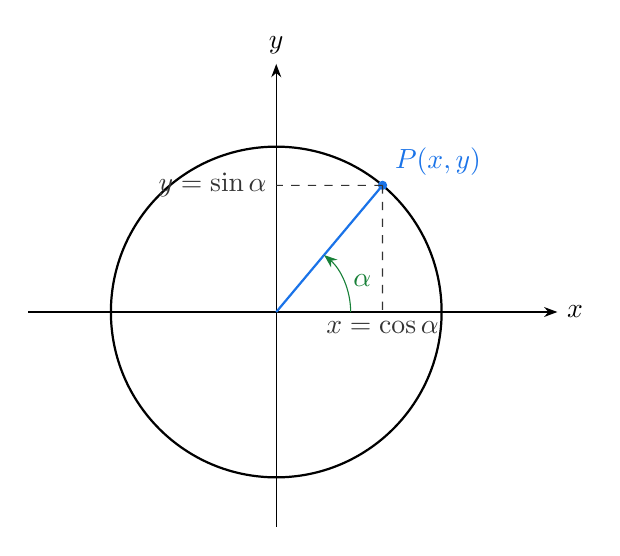
\begin{tikzpicture}[>=Stealth,scale=2.1]
  \draw[->] (-1.5,0) -- (1.7,0) node[right] {$x$};
  \draw[->] (0,-1.3) -- (0,1.5) node[above] {$y$};
  \draw[thick] (0,0) circle (1);
  \coordinate (P) at ({cos(50)},{sin(50)});
  \draw[thick,accent] (0,0) -- (P);
  \fill[accent] (P) circle (0.8pt) node[above right=0pt and 1pt] {$P(x,y)$};
  \draw[dashed,darkgray] (P) -- ({cos(50)},0) node[below] {$x=\cos\alpha$};
  \draw[dashed,darkgray] (P) -- (0,{sin(50)}) node[left] {$y=\sin\alpha$};
  \draw[->,calcframe] (0.45,0) arc (0:50:0.45) node[midway,right] {$\alpha$};
\end{tikzpicture}
\end{center}

定义立刻送三个结论：
\begin{itemize}
  \item \textbf{符号看象限}：第一象限全正；第二象限 $\sin$ 正 $\cos$ 负；第三象限全负（$\tan$ 正）；第四象限 $\cos$ 正 $\sin$ 负——不用背，看图即得；
  \item $\sin^2\alpha + \cos^2\alpha = 1$（点 $P$ 在单位圆上，$x^2 + y^2 = 1$）——这是勾股定理，不是什么新公式；
  \item \textbf{周期性}：$\alpha$ 加 $2\pi$ 终边不变，所以 $\sin(\alpha + 2\pi) = \sin\alpha$——周期性的种子在定义里。
\end{itemize}

\subsection*{8.3 诱导公式：单位圆的对称性，不是口诀表}

终边经过各种对称变换后，三角函数值怎么变？全部可以从单位圆的对称性直接读出来：
\begin{itemize}
  \item $\alpha$ 与 $-\alpha$（关于 $x$ 轴对称）：$\sin(-\alpha) = -\sin\alpha$，$\cos(-\alpha) = \cos\alpha$——正弦是奇函数、余弦是偶函数的源头；
  \item $\alpha$ 与 $\pi - \alpha$（关于 $y$ 轴对称）：$\sin(\pi-\alpha) = \sin\alpha$，$\cos(\pi-\alpha) = -\cos\alpha$；
  \item $\alpha$ 与 $\pi + \alpha$（关于原点对称）：$\sin(\pi+\alpha) = -\sin\alpha$，$\cos(\pi+\alpha) = -\cos\alpha$。
\end{itemize}

教材给了一串口诀（"奇变偶不变，符号看象限"），但每条口诀都是单位圆上的一次对称——\textbf{会画图比会背口诀可靠}。

\begin{exercise}[今日自测]
\begin{enumerate}
  \item 换算：$120°$ 等于多少弧度？$\dfrac{3\pi}{4}$ 等于多少度？
  \item $\alpha$ 是第二象限角，确定 $\sin\alpha$、$\cos\alpha$、$\tan\alpha$ 的符号。
  \item 已知 $\sin\alpha = \dfrac{3}{5}$ 且 $\alpha$ 为第二象限角，求 $\cos\alpha$ 和 $\tan\alpha$。
  \item 用单位圆解释：为什么 $\sin(30°) = \sin(150°)$？
\end{enumerate}
\end{exercise}

\newpage
% ═══ 第 9 天 ═══
\daytitle{第 9 天}{三角函数的图象、变换与应用 + 总检验}

\textbf{核心问题}：单位圆上那个点的坐标随角变化——把它"展开"成图象，长什么样？

\subsection*{9.1 正弦曲线：把单位圆展开}

让角 $\alpha$ 从 $0$ 转到 $2\pi$，单位圆上点的纵坐标 $y = \sin\alpha$ 随之上上下下。把"角"放横轴、"纵坐标"放纵轴，就描出了\textbf{正弦曲线}。五个关键点定形：

\begin{center}
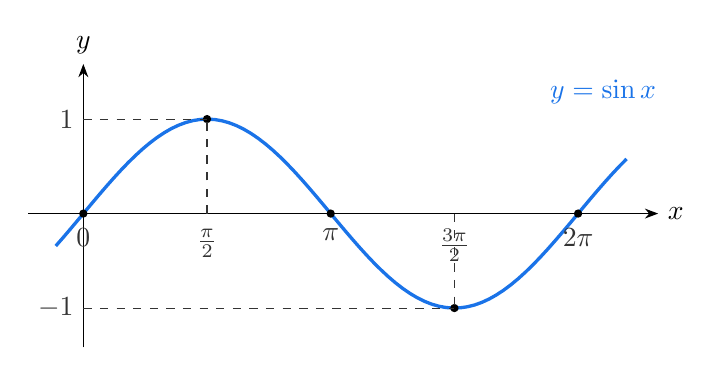
\begin{tikzpicture}[>=Stealth,scale=1.0]
  \draw[->] (-0.7,0) -- (7.3,0) node[right] {$x$};
  \draw[->] (0,-1.7) -- (0,1.9) node[above] {$y$};
  \draw[very thick,accent] plot[domain=-0.35:6.9,samples=80] (\x,{1.2*sin(\x r)});
  \node[accent] at (6.6,1.55) {$y=\sin x$};
  \foreach \p/\l/\v in {0/{0}/{0}, 1.5708/{\frac{\pi}{2}}/{1}, 3.1416/{\pi}/{0}, 4.7124/{\frac{3\pi}{2}}/{-1}, 6.2832/{2\pi}/{0}}{
    \fill (\p,{1.2*\v}) circle (1.5pt);
    \draw[dashed,darkgray] (\p,0) node[below=2pt] {$\l$} -- (\p,{1.2*\v});
  }
  \draw[dashed,darkgray] (0,1.2) node[left] {$1$} -- (1.5708,1.2);
  \draw[dashed,darkgray] (0,-1.2) node[left] {$-1$} -- (4.7124,-1.2);
\end{tikzpicture}
\end{center}

从图象和单位圆可以一起读出全部性质：
\begin{itemize}
  \item \textbf{周期性}：$T = 2\pi$（转一圈回到原点）——三角函数是高中第一支\textbf{周期函数}，描写一切周而复始：潮汐、季节、交流电、钟摆；
  \item \textbf{值域} $[-1, 1]$（单位圆的纵坐标超不过半径）；
  \item \textbf{单调性}：在 $\left[-\dfrac{\pi}{2}, \dfrac{\pi}{2}\right]$ 上增，在 $\left[\dfrac{\pi}{2}, \dfrac{3\pi}{2}\right]$ 上减；
  \item \textbf{奇偶性}：$\sin$ 是奇函数（关于原点），$\cos$ 是偶函数（关于 $y$ 轴）——第 8 天诱导公式里已经见过。
\end{itemize}
余弦曲线就是正弦曲线向左平移 $\dfrac{\pi}{2}$：$\cos x = \sin\left(x + \dfrac{\pi}{2}\right)$（单位圆里 $x$ 坐标"提前"四分之一圈达到同样高度）。

\subsection*{9.2 三角恒等变换：公式链都从单位圆长出来}

最重要的一条是\textbf{差角公式}：
\[
\cos(\alpha - \beta) = \cos\alpha\cos\beta + \sin\alpha\sin\beta
\]
它的证明只用一件事：单位圆上，角 $\alpha$、$\beta$ 对应两点的弦长，与角 $\alpha-\beta$ 对应起止点的弦长\textbf{相等}（同一个圆心角决定同一条弦），用两点间距离公式展开即得。

从这一条出发，整条公式链可以推出来，不用背：令 $\beta = -\beta$ 得和角公式；$\cos$ 换 $\sin$（用 $\frac{\pi}{2}$ 诱导）得正弦和差角；令 $\beta = \alpha$ 得\textbf{倍角公式}：
\[
\sin 2\alpha = 2\sin\alpha\cos\alpha, \qquad \cos 2\alpha = \cos^2\alpha - \sin^2\alpha
\]
学恒等变换的正确姿势：记住源头（单位圆 + 差角公式），其余随用随推。

\subsection*{9.3 $y = A\sin(\omega x + \varphi)$：三个参数，三种变换}

\[
y = A\sin(\omega x + \varphi) \qquad (A>0,\ \omega>0)
\]
\begin{itemize}
  \item $A$（\textbf{振幅}）：纵坐标伸缩 $A$ 倍——振动的"幅度"；
  \item $\omega$（\textbf{角速度}）：横坐标压缩为 $\dfrac{1}{\omega}$，周期 $T = \dfrac{2\pi}{\omega}$——振动的"快慢"；
  \item $\varphi$（\textbf{初相}）：图象左右平移——计时起点。
\end{itemize}
这个函数是物理里简谐振动的数学化身：位移、电压、声压，全是它。

\begin{center}
\begin{tikzpicture}[>=Stealth,scale=1.0]
  \draw[->] (-0.5,0) -- (7.3,0) node[right] {$x$};
  \draw[->] (0,-2.0) -- (0,2.3) node[above] {$y$};
  \draw[thick,dashed,darkgray] plot[domain=0:6.9,samples=80] (\x,{0.8*sin(\x r)});
  \node[darkgray] at (5.6,1.0) {$y=\sin x$};
  \draw[very thick,accent] plot[domain=0:6.9,samples=80] (\x,{1.6*sin(2*\x r)});
  \node[accent] at (4.5,-1.75) {$y=2\sin 2x$};
  \node[darkgray] at (3.5,-2.6) {$A$ 决定高度（振幅 2），$\omega$ 决定密度（周期 $T=\pi$）};
\end{tikzpicture}
\end{center}

\begin{exercise}[九天总检验]
\begin{enumerate}
  \item "$x > 2$"是"$x^2 > 4$"的什么条件？（充分/必要/充要）
  \item 用基本不等式求 $x(4-x)$（$0<x<4$）的最大值。
  \item 不求值，比较 $\log_2 3$ 与 $\log_4 6$ 的大小。
  \item 把 $\dfrac{5\pi}{6}$ 换算成角度，并确定它的正弦、余弦符号。
  \item 已知 $\sin\alpha = -\dfrac{4}{5}$ 且 $\alpha$ 为第三象限角，求 $\cos\alpha$。
  \item 合上本讲义，画出九天地图：集合逻辑 → 不等式 → 函数概念 → 性质 → 指数对数 → 应用 → 三角，标出每站依赖上一站的什么。
\end{enumerate}
\end{exercise}

\newpage

% ═══ 参考答案 ═══
\section*{参考答案}
\addcontentsline{toc}{section}{参考答案}

\textbf{第 1 天}
\begin{enumerate}
  \item $A \cap B = \{2,3\}$；$A \cup B = \{1,2,3,4\}$；$\complement_U A = \{4,5\}$。
  \item 充分条件。6 的倍数的集合是 3 的倍数的子集（小范围推大范围），但 3 的倍数（如 9）不一定是 6 的倍数。
  \item 否定："存在一个正方形不是矩形"——原命题为真，否定为假。
\end{enumerate}

\textbf{第 2 天}
\begin{enumerate}
  \item $-2a + 1 < -2b + 1$。$a > b$ 两边乘 $-2$ 变号得 $-2a < -2b$，再加 1 不变向。
  \item $x + \dfrac{1}{x} \geq 2\sqrt{x \cdot \dfrac{1}{x}} = 2$，当且仅当 $x = \dfrac{1}{x}$ 即 $x = 1$ 时取最小值 $2$。
  \item $x^2 - 4x + 3 > 0$：图象在轴上方，$x < 1$ 或 $x > 3$；$x^2 + x + 1 < 0$：$\Delta = 1 - 4 < 0$，抛物线恒在轴上方，无解。
\end{enumerate}

\textbf{第 3 天}
\begin{enumerate}
  \item 符合。每个 $x$ 都有唯一的 $y=1$ 与之对应——"唯一"不要求不同的 $x$ 对应不同的 $y$。
  \item 要求 $x - 2 \neq 0$ 且 $x \geq 0$，定义域为 $[0,2) \cup (2,+\infty)$。
  \item 是（定义域、对应法则都相同，字母无所谓）；是（$\sqrt{x^2} = |x|$）。
\end{enumerate}

\textbf{第 4 天}
\begin{enumerate}
  \item 任取 $x_1 < x_2$，$f(x_1) - f(x_2) = -2x_1 + 2x_2 = 2(x_2 - x_1) > 0$，故 $f(x_1) > f(x_2)$，是减函数。
  \item $f$ 偶（$f(-x) = x^4 + x^2 = f(x)$）；$g$ 奇（$g(-x) = -x^3 - x = -g(x)$）；$h$ 非奇非偶（$h(-x) = x^2 - x$，既不等于 $h(x)$ 也不等于 $-h(x)$）。
  \item $(1,1)$。因为 $1^{\alpha} = 1$ 对任何 $\alpha$ 成立。
\end{enumerate}

\textbf{第 5 天}
\begin{enumerate}
  \item $8^{2/3} = (\sqrt[3]{8})^2 = 4$；$16^{-1/2} = \dfrac{1}{\sqrt{16}} = \dfrac{1}{4}$；$\left(\dfrac12\right)^{-3} = 8$。
  \item $1.7^{0.3} < 1.7^{0.5}$（底数 $>1$，增函数）；$0.8^{0.3} > 0.8^{0.5}$（底数 $<1$，减函数）。
  \item 底数 $a > 0$ 时，$a^x$ 对任何实数 $x$ 都为正（整数次幂为正，开方取正根，逼近保持正），所以值域是 $(0,+\infty)$。
\end{enumerate}

\textbf{第 6 天}
\begin{enumerate}
  \item $3$（$2^3=8$）；$-2$（$3^{-2}=\frac19$）；$3$（$10^3=1000$）。
  \item $\log_6(2\times3) = \log_6 6 = 1$；$\log_2\dfrac{12}{3} = \log_2 4 = 2$。
  \item $x = \log_2 10$。因为 $2^3 = 8 < 10 < 16 = 2^4$，所以 $3 < x < 4$。
  \item 错。左边 $= \log_2 8 = 3$，右边 $= 2 + 2 = 4$。加法没有对数法则。
\end{enumerate}

\textbf{第 7 天}
\begin{enumerate}
  \item 有。$f(0) = -1 < 0$，$f(1) = 1 > 0$，且 $f$ 图象连续（多项式），由零点存在定理，$(0,1)$ 内必有零点。
  \item $f(0.5) = -0.375 < 0$，与 $f(1) = 1$ 异号，零点在 $(0.5, 1)$；下一次取中点 $0.75$。
  \item 指数衰减模型：剩余量 $y = a \cdot 0.9^t$（$a$ 为初始量），底数 $0.9 < 1$，递减。
\end{enumerate}

\textbf{第 8 天}
\begin{enumerate}
  \item $120° = \dfrac{2\pi}{3}$ rad；$\dfrac{3\pi}{4} = 135°$。
  \item $\sin\alpha > 0$，$\cos\alpha < 0$，$\tan\alpha < 0$（第二象限：$y$ 正 $x$ 负）。
  \item $\cos\alpha = -\sqrt{1-\sin^2\alpha} = -\dfrac{4}{5}$（第二象限取负）；$\tan\alpha = \dfrac{\sin\alpha}{\cos\alpha} = -\dfrac{3}{4}$。
  \item $150° = 180° - 30°$，两角终边关于 $y$ 轴对称，对应单位圆上点的纵坐标相同，故正弦相等（诱导公式 $\sin(\pi-\alpha) = \sin\alpha$）。
\end{enumerate}

\textbf{第 9 天（九天总检验）}
\begin{enumerate}
  \item 充分条件。$x > 2 \Rightarrow x^2 > 4$；但 $x^2 > 4$ 也可能是 $x < -2$，推不出 $x > 2$。
  \item $x(4-x) \leq \left(\dfrac{x + (4-x)}{2}\right)^2 = 4$，当且仅当 $x = 4-x$ 即 $x = 2$ 时取最大值 $4$（和定积最大）。
  \item $\log_2 3 \approx 1.58$；$\log_4 6 = \dfrac{\log_2 6}{2} \approx \dfrac{2.58}{2} = 1.29$。所以 $\log_2 3 > \log_4 6$。
  \item $\dfrac{5\pi}{6} = 150°$，第二象限角：正弦为正，余弦为负。
  \item 第三象限 $\cos\alpha < 0$，$\cos\alpha = -\sqrt{1 - \dfrac{16}{25}} = -\dfrac{3}{5}$。
  \item 集合逻辑提供语言（区间、任意/存在）$\rightarrow$ 不等式提供作差与最值工具 $\rightarrow$ 函数用集合定义 $\rightarrow$ 性质用严格定义检验（作差法、$f(-x)$）$\rightarrow$ 指数对数是具体家族（互为反函数）$\rightarrow$ 应用把方程翻译回函数（零点）$\rightarrow$ 三角用单位圆把角变成实数、把坐标变成函数，图象与公式都从单位圆长出。
\end{enumerate}

\vspace{1em}
\begin{keyconcept}[九天后，你应该能讲给别人听的六句话]
\begin{enumerate}
  \item 集合与逻辑是精确语言：确定性、互异性、无序性；小范围推大范围；否定就换量词。
  \item 基本不等式是"平方非负"的推论：算术平均 $\geq$ 几何平均，等号在相等时取到。
  \item 函数是"每个输入对应唯一输出"的规则；严格定义的灵魂是"任意"。
  \item 指数与对数互为反解：$\log_a N$ 就是"$a$ 的几次方等于 $N$"，法则都从指数法则翻译。
  \item 方程的解就是函数图象与 $x$ 轴的交点；解不出可以逼近——二分法每步把区间减半。
  \item 三角函数是单位圆上点的坐标：弧度制把角变成实数，图象、诱导公式、恒等变换都从单位圆的对称性长出来。
\end{enumerate}
\end{keyconcept}

\end{document}
